
\documentclass[10pt,a4paper]{scrartcl}

\usepackage[english]{babel}

\input{../Headerfiles/Packages}
\input{../Headerfiles/Titles}
\input{../Headerfiles/Commands}
\input{../Headerfiles/ENVIRONMENTS}
\graphicspath{{Pictures/}}
\parindent 0pt

\title{Introduction To Robotics And Mechatronics}
\author{GianAndrea Müller}

\newtheorem{define}{Definition}

\begin{document}
\begin{multicols*}{4}
\maketitle
\tableofcontents
\end{multicols*}

\begin{multicols*}{2}
\section{Basics}

\begin{define}
\textbf{Mechatronics} is defined as the field of study involving the analysis, designs, synthesis, and selection of systems that combine electronic and mechanical components with modern controls and microprocessors.
\end{define}

\begin{define}
A \textbf{Robot} is defined as an actuated mechanism programmable in two or more axes with a degree of autonomy, moving within its environment, to perform intended tasks. A robot includes the control system and interface of the control system.

\begin{itemize}
\item Perception
\item Manipulation
\item Robot-Human Interaction
\item Cognition
\end{itemize}
\end{define}

\subsection{Mechatronics Development}

\begin{define}
\textbf{Integration} must start at an early stage to make  systems less expensive, more reliable and more flexible.
\end{define}

\subsubsection{Sequential Approach}

\begin{itemize}
\item[+] Well known design process
\item[+] Centuries of experience with some systems
\item[+] Designers able to focus on specific areas
\item[-] Bulky systems
\item[-] Complex mechanisms
\item[-] Non-adjustable movement cycles
\item[-] Constant speed drives
\item[-] Mechanical synchronization
\item[-] Rigid heavy structures
\item[-] Accuracy determined by tolerance of mechanism
\item[-] Manual control
\end{itemize}

\subsubsection{Concurrent Approach}

\begin{itemize}
\item[+] Compact
\item[+] Simplified mechanisms
\item[+] Programmable movements
\item[+] Variable speed drives
\item[+] Electronics synchronization
\item[+] Lighter structures
\item[+] Accuracy achieved by feedback
\item[+] Automatic and programmable controls
\item[-] Difficult to coordinate
\item[-] More reliance on software control systems
\item[-] Broad experience needed by designers
\end{itemize}

\subsection{Robot Types}

\myspic{0.7}{Pictures/RobotTypes}

\section{Labs}

\subsection{00}

A hexadecimal number is a number expressed by a base-16 numeral system which uses the symbols 0-9 and A-F. For conversion between hexadecimal and decimal apply the algorithms learned for binary numbers. On preference convert to binary first, using hex nibbles.

\subsubsection{Binary number formats}

\begin{TTable}{ll}
Name&Size (bits)\\
Bit&1\\
Nibble&4\\
Byte&8\\
Word&16\\
Double Word&32\\
\end{TTable}

\subsubsection{Conversion from Decimal to other systems}

\paragraph{Dividing by the base}

Dividing the decimal number by the base of the target positional notation system and recording the resulting remainders until the integer part results in 0 delivers the digits of the number in reverse order.

\begin{center}
\begin{tabular}{lll}
Quotient&Integer Part&Remainder\\
18435/16&1152&3\\
1152/16&72&0\\
72/16&4&8\\
4/16&0&4\\
\end{tabular}
\end{center}

\paragraph{Subtraction Method}

Start with a weighted position greater than the number.

\begin{itemize}
\item If the number is greater than the weighted position for the digit, write down a 1 and subtract the weighted position value.
\item If the number is less than the weighted position for the digit, write down 0 and subtract 0.
\end{itemize}

\subsubsection{Hex Nibbles}

Any of the hexadecimal digits can be understood as a nibble (4 bits). Therefore hexadecimal numbers can be viewed as a compact representation of binary numbers, since every hexadecimal bit directly translates to a certain nibble as listed below.

\begin{TTable}{lll|lll}
hex&bin&dec&hex&bin&dec\\
0&0000&0&8&1000&8\\
1&0001&1&9&1001&9\\
2&0010&2&A&1010&10\\
3&0011&3&B&1011&11\\
4&0100&4&C&1100&12\\
5&0101&5&D&1101&13\\
6&0110&6&E&1110&14\\
7&0111&7&F&1111&15\\
\end{TTable}

\subsubsection{Two's Complement}

Writing negative numbers in the two's complement does not simply use the first bit in a binary number as a sign bit, but assigns that bit its negative positional value. Thereby the double-encoding of 0 (negative 0 respectively) is omitted.

\begin{TTable}{lll|lll}
\multicolumn{6}{c}{\textbf{Two's complement}}\\
Bits&Unsigned value&2's&Bits&Unsigned value&2's\\
0000&0&0&1000&8&-8\\
0001&1&1&1001&9&-7\\
0010&2&2&1010&10&-6\\
0011&3&3&1011&11&-5\\
0100&4&4&1100&12&-4\\
0101&5&5&1101&13&-3\\
0110&6&6&1110&14&-2\\
0111&7&7&1111&15&-1\\
\end{TTable}

\paragraph{How to find the Two's Complement Representation}

\begin{enumerate}
\item Find the binary representation of the magnitude of the number.
\item Find the binary complement of that representation. Flipping 0 to 1 and vice versa.
\item Add one to the complement.
\end{enumerate}

The above method applied to hexadecimal numbers requires the conversion to binary and back. This can be circumvented using the following approach:

\begin{enumerate}
\item Subtract each hexadecimal digit from 15.
\item Add 1 to the resulting number.
\end{enumerate}

\subsubsection{Declaring numbers in C}

\begin{TPCpp}
#include <stdint.h>
uint16_t a = 0x4803;
\end{TPCpp}

Since the built in data types of C are ambiguous, depending on the system used on. For that reason \verb+stdint.h+ is used, making the following data types available:

\begin{TTable}{cccc}
Type declaration&Bits&Type&Range\\
int8\_t&8-bit&integer&-128 - 127\\
uint8\_t&8-bit&unsigned integer&0 - 255\\
int16\_t&16-bit&integer&-32768 - 32767\\
uint16\_t&16-bit&unsigned integer&0 - 65535\\
int32\_t&32-bit&integer&-2'147'483'648 - 2'147'483'647\\
uint32\_t&32-bit&unsigned integer&0 - 4'294'967'295\\
int64\_t&64-bit&integer&-9.22$\cdot 10^{18}$ - 9.22$\cdot10^{18}$\\
uint64\_t&64-bit&unsigned integer&0 - $1.84\cdot10^{19}$\\
\end{TTable}

\subsubsection{Bitwise Operators}

Bitwise operators work on bits and perform bit-by-bit operations. The truth tables for bitwise AND \verb.&., bitwise OR \verb.|. and bitwise exclusive OR (XOR) \verb.^. are:

\begin{TTable}{*{5}{c}}
\verb.p.&\verb.q.&\verb.p&q.&\verb.p|q.&\verb.p^q.\\
0&0&0&0&0\\
0&1&0&1&1\\
1&1&1&1&0\\
1&0&0&1&1\\
\end{TTable}

\begin{TTable}{lp{0.8\linewidth}}
\verb.&.&Binary AND Operator copies a bit to the result if it exists in both operands.\\
\verb.|.&Binary OR Operator copies a bit if it exists in either operand.\\
\verb.^.&Binary XOR Operator copies the bit if it is set in one operand but not both.\\
\verb.~.&Binary Ones Complement Operator is unary and has the effect of 'flipping' bits.\\
\verb.<<.&Binary Left Shift Operator. The left operands value is moved left by the number of bits specified by the right operand.\\
\verb.>>.&Binary Right Shift Operator. The left operands value is moved right by the number of bits specified by the right operand.\\
\end{TTable}

\subsection{05 - Lessons in Debugging}

\begin{enumerate}
\item Reboot.
\item Check all wire connections thoroughly.
\item Check if the hardware is functional.
\item Check if all variables are initialized.
\item Check if the array size is correct.
\item Check initial conditions for loops.
\item Check incrementation for loops.
\item Check for potential segmentation faults.
\begin{itemize}
\item For example advancing over array in the wrong direction.
\end{itemize}
\item Check for integer divisions.
\item Check result reproducibility to detect random successes.
\item Output values, include unit tests.
\item Check superfluous semicolons.
\item Empty trash to avoid file conflicts.
\end{enumerate}

\subsubsection{OpenCV}

\begin{itemize}
\item Check if all images are closed \verb+cVReleaseImage(&image_name);+
\item Check if all captures are closed \verb+cVReleaseCapture(&capture_name);+
\item Check if all files are closed \verb+fclose(file_name);+
\end{itemize}

\section{Linux Commands and C Basics}

\subsection{Basic File Manipulations}

\begin{TTable}{lll}
Command&Function&MSDOS Equivalent\\
cp&Copy a file or collection of files&COPY\\
mv&Move or rename a file or collection of files&COPY REN\\
rm&Remove a file or collection of files&DEL\\
ln&Create a link (or alias) from one file to another&N/A\\
ls&List a directory. There are a lot of options&DIR\\
mkdir&Create a directory&MKDIR\\
rmdir&Remove a directory (must be empty)&RMDIR\\
\end{TTable}

\subsection{File naming}

\begin{itemize}
\item Maximum name length: 255, the path can be longer,.
\item All characters besides \verb+'/'+ and NUL are allowed. 
\item File names are case sensitive.
\item File names do not have components or extensions. Many applications however regard the part of a file name after the last dot as having special significance.
\end{itemize}

\subsection{Wildcards}

\begin{TTable}{lp{0.8\linewidth}}
\verb+*+&Matches any sequence of characters.\\
\verb+?+&Matches any single character.\\
\verb+[..]+&Matches any of the characters included in the list between the brackets. Ranges may also be specified using a dash so, for example \verb+[a-z]+ means any lower case letter.\\
\verb+[!..]+&Matches any character not included in the list.\\
\end{TTable}

\subsection{Escaping Conventions}

\begin{TTable}{ll|ll}
\verb+*+&File naming wild card&\verb+?+&File naming wild card\\
\verb+[+&File naming wild card&\verb+]+&File naming wild card\\
\verb+$+&Shell variable substitution&\verb+&+&Shell backgrounding\\
\verb+<+&Input rederection&\verb+>+&Output rederection\\
\verb+|+&Shell piping&\verb+;+&Shell command grouping\\
\verb+(+&Shell command grouping&\verb+)+&Shell command grouping\\
\verb+{+&Shell variable substitution&\verb+}+&Shell variable substitution\\
\verb+\+&Shell escaping&\verb+"+&Shell escaping\\
\verb+`+&Shell escaping&\verb+'+&Shell command substitution\\
\end{TTable}

In addition \verb+^+ and \verb+!+ can cause problems when used in file names. Files beginning with \verb+-+ are also problematic.

It is possible to overcome many of the constraints by escaping file names containing awkward characters using quotes to enclose them or preceding awkward characters with a backslash.

\subsection{Compilation}

\begin{TTable}{lp{0.5\linewidth}}
\verb+gcc anyname.c+&Compile a program in c with any name desired.\\
\verb+cc myprog.c+&Compile a program in c called myprog.\\
\verb+cc myprog.c 2>myprog.errs+&Capturing compilation errors.\\
\verb+cc -o myprog myprog.c+&Specific output file name.\\
\verb+cc -o myprog myprog.c -lm -ls626+&Inclusion of math and sensoray libraries.\\
\verb+cc -c green.c+&Stop compilation after the assembler stage, producing \verb+green.o+.\\
\end{TTable}

\paragraph{Separate compilation steps}

\begin{enumerate}
\item Compile green.o: \verb+cc -c green.c+
\item Compile blue.o: \verb+cc -c blue.c+
\item Link the parts together: \verb+cc green.o blue.o+
\end{enumerate}

\paragraph{Splitting a program}

\begin{itemize}
\item Be sure no two files share function names.
\item Be sure no two files share global variable names.
\item Declare global variables in the header file: \verb+extern int globalvar+.
\item To use functions from another file make a .h file with the function prototypes and use \verb+#include+ to include those .h files within your c files.
\item At least one of the files must have a main() function.
\end{itemize}

\subsubsection{Variable Definition}
\label{sec:VariableDefinition}

A variable definition tells the compiler where and how much storage to create for the variable. A variable definition specifies a data type and name. Multiple names can be introduced at once if separated by commas.

\begin{TPCpp}
int i,j,k;
\end{TPCpp}

This line both declares and defines the variables i,j and k.
Direct initialization is also possible:

\begin{TPCpp}
int d = 3, f = 2;
\end{TPCpp}

\textbf{If a variable is left uninitialized its value is undefined in general}. However, variables with static storage duration are implicitly set to 0.

\subsubsection{Variable Declaration}

It is possible to declare a variable without defining it. The declaration is accepted during compilation but has to be fitted with a definition at the time of linking of the program. This means that if a program consists of multiple files you can declare your variable wherever you need it but only define it once, since multiple definitions of the same variable are prohibited.

\begin{TPCpp}
//Variable declaration (everywhere needed)
extern int a,b; //Compiler knows that the variable exists

//Variable definition (only once)
int a,b; //Compiler knows that the variable exists
         //And allocates the storage space needed
\end{TPCpp}

\subsection{Dependencies and Makefiles}

\myspic{1}{Pictures/Dependencies}

A makefile encodes the dependencies of different parts of the program, enabling building the code in an optimized manner by only compiling the part of the dependency tree that was affected by a change. Note that only files listed in the makefile will lead to an update when changed. In the example above changing the .h-files for example will not do that.

\begin{TPCpp}
make //will execute 'Makefile' or 'makefile'
make -f otherfile //accepts any filename
\end{TPCpp}

\subsubsection{Macros in make}

\begin{TPCpp}
OBJECTS = data.o main.o io.o
project1: $(OBJECTS)
	cc $(OBJECTS) -o project1
data.o: data.c data.h
	cc -c data.c
main.o: data.h io.h main.c
	cc -c main.c
io.o: io.h io.c
	cc -c io.c
\end{TPCpp}

A macro can also be specified when running make. This overrides the value of OBJECTS within the above specified makefile.

\begin{TPCpp}
make 'OBJECTS=data.o newio.o main.o' project1
\end{TPCpp}

\paragraph{Special macros}

\begin{itemize}
\item \verb+CC+ Contains the current C compiler. Defaults to cc.
\item \verb+CFLAGS+ Special options which are added to built-in C rule.
\item \verb+$@+ Full name of the current target.
\item \verb+$?+ A list of files for current dependency which are out-of-date.
\item \verb+$<$+ The source file of the current (single) dependency.
\end{itemize}

\paragraph{Manipulate macro evaluation}

Assuming \verb+OBJS=data.o io.o main.o+ the macro can be reinterpreted using

\begin{TPCpp}
$(OBJS:.o=.c) //data.c io.c main.c
\end{TPCpp}
%$

\paragraph{Predefined rules}

make knows that to create an .o file the corresponding .c file is needed. Thus these .c files can be omitted. \textcolor{red}{Why are the corresponding make commands not repeated?}

\begin{TPCpp}
OBJECTS = data.o main.o io.o
project1: $(OBJECTS)
	cc $(OBJECTS) -o project1
data.o: data.h
main.o: data.h io.h
io.o: io.h
\end{TPCpp}

When compiling programs on Wiliki add on top:

\begin{TPCpp}
CFLAGS=-Aa -D_HPUX_SOURCE
\end{TPCpp}

which allows make to use ANSI standard C compilation.

\paragraph{Shortcuts}

There can be more than one file in the target section of the dependency rules. If a file appears in several target sections all its sources are gathered.

\begin{TPCpp}
CFLAGS = -Aa -D_HPUX_SOURCE
OBJECTS = data.o main.o io.o
project1: $(OBJECTS)
	cc $(OBJECTS) -o project1
data.o main.o: data.h
io.o main.o: io.h
\end{TPCpp}

\subsection{Pointers and Structures}

\begin{TPCpp}
struct tag {
	char lname[20]; /* last name */
	char fname[20]; /* first name */
	int age; /* age */
	float rate; /* e.g. 12.75 per hour */
};
\end{TPCpp}

The following file declares an instance of the structure, assigns data and then prints it out.

\begin{TPCpp}
struct tag my_struct; /* declare the structure my_struct */
int main(void)
{
strcpy(my_struct.lname,"Jensen");
strcpy(my_struct.fname,"Ted");
printf("\n%s ",my_struct.fname);
printf("%s\n",my_struct.lname);
return 0;
}
\end{TPCpp}

\begin{itemize}
\item In original C we cannot pass whole structures to functions, in ANSI standard C however that is possible.
\end{itemize}

\begin{TPCpp}
struct tag *st_ptr; //declare a pointer to type <struct tag>
st_ptr = &my_struct; //let it point to the above instance
(*st_ptr).age = 63; //dereference it for access
st_ptr->age = 63; //dereferencing and access in one
\end{TPCpp}

\subsection{Arithmetic Conversion}

Whenever an arithmetic operator encounters variables of different types they are cast to a common type following the hierarchy below:

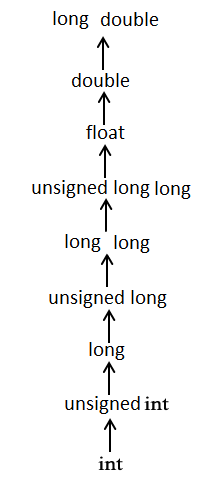
\includegraphics[angle=90, width=\linewidth]{UsualArithmeticConversion}

\section{Sensors}

\begin{define}
\textbf{Range} The \textbf{range} of a sensor defines the limits between which the input can vary.
\end{define}

\begin{define}
The \textbf{span} of a sensor is the maximum value of the input minus the minimum value.
\end{define}

\begin{define}
The \textbf{sensitivity} of a sensor is a relationship that indicates how much output per unit input the sensor produces.
\end{define}

\begin{define}
The \textbf{accuracy} of a sensor captures the extent to which the values indicated by a measurement system might be wrong.
\end{define}

\begin{define}
The \textbf{repeatability} of a sensor describes its ability to give the same output for repeated applications of the same input value.

\mportant{repeatability = $\frac{\text{value}_{max}-\text{value}_{min}}{\text{range}}\cdot 100$}
\end{define}

\mypic{Repeatability}

\begin{define}
The \textbf{resolution} of a sensor is the smallest change in the input value that will produce an observable change in the output.
\end{define}

\begin{define}
The \textbf{stability} of a sensor is its ability to give the same output when used to measure a constant input over a period of time.

\textbf{Drift} is often used to describe the change of output over time.

\textbf{Zero drift} is used of changes that occur in output when there is zero input.
\end{define}

\begin{define}
The \textbf{error} describes the difference between the result of the measurement and the true value of the quantity being measured.
\end{define}

\begin{define}
The \textbf{hysteresis error} describes the difference between two measurements of the same value once measured on an increasing and once measured on a decreasing change.
\end{define}

\begin{define}
The \textbf{non-linearity error} describes how much error arises from the assumption that the transducer has a linear relationship between input and output.
\end{define}

\begin{define}
The \textbf{static characteristics} of a sensor describe its behaviour in the steady state.
\end{define}

\subsection{Dynamic Characteristics}

\begin{define}
The \textbf{dynamic characteristics} of a sensor describe its transient behaviour before reaching the steady state.\end{define}

\begin{define}
The \textbf{response time} of a dynamic system is the time that elapses after a constant input is applied until a certain percentage of the input is reached.
\end{define}

\begin{define}
The \textbf{time constant} of a dynamic system is a measure of the inertia. It describes how fast the system reacts. The larger the time constant, the slower the reaction.
\end{define}

\begin{define}
The \textbf{rise time} of a dynamic system is the time that elapses after until the output rises to some specified percentage of the steady-state output. 
\end{define}

\begin{define}
The \textbf{settling time} is the time taken for the output to settle to within some percentage of the steady-state value.
\end{define}

\subsection{Sampling}

\importname{Nyquist's Sampling Theorem}{$f_s>2 f_{\max}$}

\begin{TDefinitionTable*}
$f_s$&Sampling rate&$\si{\hertz}$\\
$2 f_{\max}$&Nyquist frequency&$\si{\hertz}$\\
\end{TDefinitionTable*}

\subsubsection{Analog-to-digital Conversion}

\begin{enumerate}
\item Quantization: Transformation of a continuous analog signal into a set of discrete output states.
\item Coding: Assignment of digital codes to each output state.
\end{enumerate}

\begin{define}
\textbf{Resolution} of an ADC is the number of bits used to approximate the analog value of the input.

\important{$N=2^n$}

\begin{TDefinitionTable*}
$N$&Number of possible states\\
$n$&Number of bits\\
$N-1$&Number of decision points\\
\end{TDefinitionTable*}

The \textbf{maximum error} is $\pm 1/2$ LSB (\textbf{Least Significant Bit}).
\end{define}

\myspic{0.6}{Coding}

\begin{define}
The \textbf{aperture time} is the time window during which the output has any error due to changes of the input.
\end{define}

\begin{define}
\textbf{Dithering} is the process of adding random noise to a signal before discretizing it order to randomize the quantization error. 
\end{define}

\subsubsection{Digital-to-Analog Conversion}

\begin{itemize}
\item Inmpulse train
\begin{itemize}
\item[-] Difficult to do exactly in electronics
\item[-] Does not preserve original spectrum
\end{itemize}
\item Sample and hold
\begin{itemize}
\item Equivalent to sample and hold from ADC
\end{itemize}
\end{itemize}

\begin{define}
A \textbf{reconstruction filter} is used to create a smooth analog signal from the digital output of a DAC.
\end{define}

\subsection{Signal Analysis}

\begin{define}
The \textbf{mean} is the average of a signal an correspond to the DC current of a signal.

\mportant{$\mu=\expe{X}=\frac{1}{N}\sum\limits_i x_i=\sum\limits_{-\infty}^\infty x PDF(x)dx$}
\end{define}

\begin{define}
The \textbf{standard deviation} $\sigma$ describes how far the $i^{th}$ sample deviates from the mean.

\begin{align*}
\sigma^2&=\expe{(X-\mu)^2}\\
&=\frac{1}{N-1}\sum\limits_i (x_i-\mu)^2\\
&=\int_{-\infty}^\infty (x-\mu)^2 PDF(x)dx
\end{align*}

$\sigma^2$ is called the \textbf{variance} of the signal.
\end{define}

\begin{define}
The \textbf{signal to noise ratio (SNR)} is defined as

\mportant{$SNR=\frac{\mu}{\sigma}$}
\end{define}

\begin{define}
The \textbf{coefficient of variation (CV)} is defined as

\mportant{$CV=\frac{\sigma}{\mu}100\%$}
\end{define}

\importname{Normal Distribution}{$P(x)=\frac{1}{\sqrt{2\pi}\sigma}e^{-(x-\mu)^2/2\sigma^2}$}

\section{Signal Processing}

\begin{define}
\textbf{Noise} can be described as an undesired disturbance in a measurement signal.
\end{define}

Noise can be caused by
\begin{itemize}
\item Mechanical Vibrations and Acoustic Sources
\item Thermal effects
\item Electrical effects
\begin{itemize}
\item \textbf{Shot (Schottky) Noise} arises due to non-continuous or quantized nature of electron transport. Stops when current flow stops, has flat PSD, is independent of temperature.

\mportant{$I_n=\sqrt{2qI_{dc}\Delta\omega}$}
\item \textbf{Johnson-Nyquist Noise} is caused by thermal agitation of electrons at thermal equilibrium.
\mportname{\\Voltage Variation per root hertz bandwith}{$V_n=\sqrt{4k_BTR}$ in $\si{\volt}/\sqrt{\si{\hertz}}$}
\end{itemize}
\item Quantization effects (maximum error of $\pm \frac{1}{2}$ LSB)
\item Numerical effects (fixed number of bits, representation errors)
\begin{itemize}
\item Additive error increases with $N$
\item Random error increases with $\sqrt{N}$
\end{itemize}
\end{itemize}

\subsection{Signal Conditioning}

\textbf{Reasons for conditioning:}
\begin{itemize}
\item Correct magnitude and phase
\item Amplification
\item Interference Removal
\item ADC, DAC
\item Safety
\end{itemize}

\textbf{Examples:}

\begin{itemize}
\item Fuses to prevent damage to the next element
\item Circuit isolations (opto-couplers) delivering information encoded as light
\item Polarity protection
\item Voltage limitation
\end{itemize}

\subsection{Signal Amplification}

\subsubsection{Ideal Amplifier (Opamp)}

\myspic{0.6}{Opamp}

\begin{itemize}
\item Infinite impedance at inputs $I_+ = I_-=0$
\item Infinite gain $V_0=K_{\rightarrow\infty}(V_+-V_-)$
\item Zero input impedance
\item Closed loop gain: $K_{closed} = \frac{K_{open}}{1+K_{open}\cdot Feedback}$

where $Feedback$ denotes how much of the output signal (in percent) is fed back.
\item Closed loop gain for large open loop gains: $K_{closed}=\frac{1}{Feedback}$
\end{itemize}

\myspic{0.6}{Amps}

\subsection{Signal Filtering}

\begin{define}
\textbf{Filtering} is used to describe the process of removing a certain band of frequencies from a signal and permitting others to be transmitted.
\end{define}

\begin{define}
A \textbf{passive filter} is built only from resistors, capacitors and inductors.

An \textbf{active filter} also includes operational amplifiers.
\end{define}

\begin{define}
\textbf{Digital filtering} describes the process of filtering the signal after it has been sampled.
\end{define}

Check out the lecture for details on Fouriertransform, Laplacetransfrom, Time vs. Frequency domain and the implementation of a range of basic filters.

\section{Digital Filtering}

\begin{define}
\textbf{Filters} are used for signal restoration (removal of unwanted parts of the signal such as noise) and signal separation (extraction of useful parts of the signal).
\end{define}

\begin{itemize}
\item Analog filters
\begin{itemize}
\item[+] Cheap
\item[+] Fast
\item[+] Have a large dynamic range in amplitude and frequency
\end{itemize}
\item Digital filters
\begin{itemize}
\item[+] Programmable / Versatile
\item[+] Can handle slow signals
\item[+] No drift / temperature dependency
\item[-] Introduce a delay into the signal (more components in the signal path)
\item[-] Relatively expensive
\item[-] Not impervious to noise
\end{itemize}
\end{itemize}

\textbf{Filtering approaches}
\begin{itemize}
\item \textbf{Convolution}: Weighted average of samples of the input. 
\item \textbf{Recursion} Weighted average of samples of the input and previously calculated samples of the output.
\end{itemize}

\textbf{Filter characteristics}

\begin{define}
\textbf{FIR} filters have a finite impulse response, thus the response settles to zero in finite time. 

\begin{itemize}
\item[+] Require no feedback, thus rounding errors are not accumulated and the computation is simpler.
\item[+] Inherently stable.
\item[+] When having a symmetric coefficient sequence they automatically have linear phase.
\item[-] Need more computation power, especially for low frequency cutoffs.
\end{itemize}
\end{define}

\begin{define}
\textbf{IIR} filters have a frequency response that continues infinitely. Analog filters (resistance, capacitors / inductors) are generally IIR filters.

\begin{itemize}
\item[+] Efficiently implemented for certain requirements (passband, stopband, ripple, roll-off). The same requirements can be met with a lower order IIR than FIR.
\item[+] Efficient calculation
\item[-] Harder to design
\item[-] Nonlinear phase likely, linear phase only approximately achievable
\end{itemize}
\end{define}

\begin{define}
A filter with a \textbf{linear phase} has a linear dependency between frequency and phase response.
\end{define}

\begin{define}
A filter with a nonlinear phase can have \textbf{phase distortion}, which leads to a change in the shape of the waveform.
\end{define}

\begin{define}
\textbf{Stopband attenuation} describes how fast the filters response decays for frequency above the passband.
\end{define}

\begin{itemize}
\item[+] Fast step response
\item[+] No overshoot
\item[+] Linear phase (no phase distortion)
\item[+] Fast roll-off
\item[+] No ripple in passband
\item[+] Good stopband attenuation
\end{itemize}

\subsection{Moving Average}

\myspic{0.7}{Pictures/Sinc}

The inverse fourier transform of the ideal frequency response produces a sinc function.

\mportant{$h[i]=\frac{\sin(2\pi f_c i)}{i\pi}$}

This is easily calculated but not so easily implemented on a computer since it is infinite in time. The solution is to apply a smooth window to the time domain signal in order to avoid an abrupt ending of the IR of the filter. For that purpose Blackman or Hann Windows are applied.

\section{Actuators}

\subsection{Hydraulics}

\begin{itemize}
\item[+] High power/weight ratio
\item[+] Low time constants
\item[+] High stiffness due to fluid incompressibility
\item[-] High cost due to the hydraulic system
\item[-] Space requirements lead to difficult miniaturization
\item[-] Risk of oil leaks (messy)
\end{itemize}

\subsection{Pneumatics}

\begin{itemize}
\item[+] Availability and cleanliness of air
\item[+] Leaks are not dangerous
\item[-] Lower energy density than hydraulics
\item[-] Compressibility of air leads to imprecise kinematic control
\end{itemize}

\subsection{Specific Energy}

\begin{define}
The \textbf{specific energy} of an actuator refers to the amount of energy it can produce in a given volume.
\end{define}

For pneumatic/hydraulic actuators the specific energy corresponds to the pressure: $w_{hdy}=w_{pne}=p$, for electrochemical actuators the specific energy is: $w_e=\frac{1}{2}B^2/\mu_0$.

\begin{tabular}{|l|l|l|}
Type&Limiting factor&Specific energy\\
Hydraulic&$p_{max}=\SI{70}{\bar}$&$\SI{7e6}{\joule\per\meter\cubed}$\\
Pneumatic&$p_{max}=\SI{6}{\bar}$&$\SI{0.6e6}{\joule\per\meter\cubed}$\\
Electric&$B_s=\SI{1}{\tesla}$&$\SI{0.4e6}{\joule\per\meter\cubed}$
\end{tabular}

where $B_s$ corresponds to the saturated magnetic field.

\subsection{Solenoid}

\begin{define}
A \textbf{solenoid} consists of a coil and a movable iron core called \textbf{armature}. A solenoid can act as a  relay when establishing an electrical contact.
\end{define}

\subsection{Voice Coil}

\begin{define}
A \textbf{voice coil} consist of a coil that moves in a magnetic field produced by a permanent magnet and intensified by an iron core.
\end{define}

\subsection{Material deformation actuation}

\begin{itemize}
\item[+] High energy density
\item[+] High rigidity
\item[+] High resolution
\item[-] Small deformations (mechanical amplification necessary)
\end{itemize}

Possible approaches
\begin{itemize}
\item Thermal deformation through resistive heating
\item Conducting polymers
\begin{itemize}
\item[+] High force
\item[+] High deformations
\item[-] Low frequencies
\end{itemize}
\item Magnetostriction
\item Shape memory alloys (switching between different crystalline structures through heating
\item Piezo drives
\begin{itemize}
\item[+] Can be used to generate displacement/force or a combination of both
\end{itemize}
\mportant{$F_{max}\approx k_T\Delta L_0$}

\mportant{$F_{max,eff}\approx k_T\Delta L_0\left(1-\frac{k_T}{k_T+k_S}\right)$}

\begin{TDefinitionTable*}
$\Delta L_0$&maximal nominal displacement\\
$k_T$&piezo actuator stiffness\\
$k_S$&external spring stiffness (environment)\\
\end{TDefinitionTable*}
\item Slip-Stick Actuator

A piezo actuator is attached to a mobile base. It slowly extends while the base remains stationary and retracts quickly such that the base slips.

\mportant{$v=(L-\delta)f$}

\begin{TDefinitionTable*}
$v$&velocity
$f$&frequency\\
$L$&full elongation\\
$\delta$&backlash\\
\end{TDefinitionTable*}

\end{itemize}

\subsection{Electric Motors}

\begin{itemize}
\item Brushless (vs. Brushed)
\begin{itemize}
\item[+] High power density
\item[+] Easier manufacture
\item[+] Less wear/tear, low heat generation
\item[+] Quicker speed adjustment with electronic control
\end{itemize}
\item Induction Motor
\begin{itemize}
\item[+] Simple and low-cost construction
\item[+] Low maintenance costs
\item[+] Can be used in hazardous environments, since it produces no sparks
\end{itemize}
\item Servomotor
\begin{itemize}
\item[+] Precise control of displacement, velocity and acceleration
\item[+] Incorporates closed-loop servomechanism
\end{itemize}
\item Stepper
\begin{itemize}
\item[+] Simple construction
\item[+] Open loop control (no position sensor necessary
\item[+] High starting torque
\item[+] Can rotate in both directions
\item[+] Can move in precise angular increments
\item[-] Slip if overloaded
\item[-] Preferential stopping positions
\item[-] Vibrations
\item[-] Low maximal speed
\end{itemize}
\end{itemize}

\mportname{\\Back electromotive force (EMF)}{$V_{emf}=k_e\omega$}

\important{$V_{in}=\underbrace{L\frac{d I_{in}}{dt}}_{\text{neglectable}}+RI_{in}+k_e\omega$}

\important{$T=k_tI_{in}$}

\begin{TDefinitionTable*}
$k_e$&electrical motor constant\\
$k_t$&torque motor constant\\
\end{TDefinitionTable*}

\important{$T=\left(\frac{k_t}{R}\right)V_{in}-\left(\frac{k_ek_t}{R}\right)\omega$}

\mportant{$T(\omega)=T_s\left(1-\frac{\omega}{\omega_{max}}\right)$}

\begin{TDefinitionTable*}
$T_s$&Stall torque ($\omega = 0$)\\
$\omega_{max}$&No-load speed ($T=0$)\\
\end{TDefinitionTable*}

\mportant{$T_s=\left(\frac{k_t}{R}\right)V_{in}\qquad \omega_{max}\frac{T_sR}{k_ek_t}$}

\important{$P(\omega)=T\omega=\omega T_s\left(1-\frac{\omega}{\omega_{max}}\right)$}

The maximum power is obtained at $\omega^\ast =\frac{1}{2}\omega_{max}$.

\subsection{Gearheads}

\begin{itemize}
\item Spur gearhead
\begin{itemize}
\item[+] Low friction per train
\item[+] Input and output shaft need not be aligned
\item[-] Low torque
\end{itemize}
\item Planetary gearhead
\begin{itemize}
\item[+] Higher reduction ratio per train and higher friction
\item[+] Higher torques
\item[+] High performance in small space
\end{itemize}
\end{itemize}

\mportant{$\omega_{load}=\frac{1}{r}\omega_{motor}\qquad T_{load} = r T_{motor}\qquad J^{equ}_{motor}=\frac{1}{r^2}J_{load}$}

\begin{TDefinitionTable*}
$r$&gear ratio\\
$J$&inertia\\
\end{TDefinitionTable*}

The optimal gear ratio for load acceleration and for minimizing the dissipated energy is:

\mportant{$r_{opt} = \sqrt{\frac{J_{load}}{J_{motor}}}$}

\begin{align*}
P_{input} &= V_{in}\cdot I_{in}\\
P_{output} &= T\omega\\
P_{loss} &= T_{friction}\omega + R_{a}I^2
\eta&=\frac{P_{output}}{P_{input}}
\end{align*}

\section{Computer Vision}

\begin{define}
A \textbf{camera} is a device comprising optics, an imaging sensor, digitization hardware and optionally computer vision algorithms reproducing a view of the world.
\end{define}

\subsection{Sensor technologies}

\begin{itemize}
\item \textbf{CCD} (Charged Coupled Device) 
\begin{itemize}
\item[+] High sensitivity
\item[+] High dynamic range
\item[-] Expensive
\item[-] Needs off-chip circuitry
\end{itemize}
\item \textbf{CMOS} (Complementary Metal-Oxide Semiconductor)
\begin{itemize}
\item[+] All electronics on a single chip
\item[+] Much cheaper
\end{itemize}
\end{itemize}

\subsection{Color Cameras}

\myspic{0.7}{Pictures/ColorImages}

\section{Robot Kinematics}

\begin{define}
The \textbf{Degrees of Freedom (DOF)} of a robotic system defines the number of independent movements the system can perform with respect to a coordinate system.
\end{define}

\begin{define}
The \textbf{forward kinematics} of a robotic system describe the position and orientation of the end effector depending on the joint angles.
\end{define}

\begin{define}
The \textbf{inverse kinematics} of a robotic system describe the joint angles depending on a desired end effector position.
\end{define}

\begin{define}
A \textbf{redundant robot} has more joints than the DOF of the task space.
\end{define}

\important{$\begin{bmatrix}
\dot{x}_{1,ee}\\\vdots\\\dot{x}_{n,ee}
\end{bmatrix}=\vec{J}\begin{bmatrix}
\dot{q}_1\\\vdots\\\dot{q}_n
\end{bmatrix}$}

\begin{TDefinitionTable*}
$\vecd{x}_ee$&velocity of the end effector\\
$\vecd{q}$&joint velocities\\
$\vec{J}$&Jacobian\\
\end{TDefinitionTable*}

\begin{define}
A \textbf{path} is a locus of points in the task space is a purely geometric description of motion.

A \textbf{trajectory} is a path on which a time law is defined. It is a spatio-temporal description of motion.
\end{define}

\subsection{Control}

A simple approach to controlling a multi-degree of freedom robot is controlling each joint separately.

\section{Modelling and Control of Dynamic Systems}

Laplace Transform:

\importabflex{c}{$L_t\left[f(t)\right](s)\equiv\int_0^\infty f(t)e^{-st}dt$\\$f(t)\equiv \frac{1}{2\pi j}\int_{\sigma-j_\infty}^{\sigma+j_\infty}F(x)e^{st}ds$}

Properties
\begin{itemize}
\item Linearity
\item First derivative
\mportant{$L_t\left[\ddt f(t)\right]=sF(x)-f(0)$}
\item Second derivative
\mportant{$L_t\left[\frac{d^2}{dt^2} f(t)\right]=s^2F(s)-sf(0)-\ddt f(0)$}
\item Integral
\mportant{$L_t\left[\int f(t)dt\right]=\frac{1}{s} F(s)$}
\end{itemize}

%insert list of important laplace transform pairs

\subsection{Standard test signals}

\myspic{0.7}{Pictures/TestSignals}

\subsection{DC Motor Transfer Function}

\importabflex{c}{$V_{armature}=L\frac{d I_{armature}}{dt}+RI_{armature}+K_{backemf}\omega,\quad (K_{backempf}\omega = e_b)$\\$V(s)=(sL+R)I(s)+K_bs\Theta$\\$I(s)=\frac{V(s)-sK_b\Theta}{Ls+R}$\\$\Theta(s)=\frac{K_t I(s)}{s(Js+b)}$}

neglecting the armature inductance:

\mportant{$\frac{\Theta(s)}{V(s)}=\frac{K_t}{s^2RJ+s(Rb+K_tK_b)}$}

where we define $K_m = K_t(Rb+K_tK_b)$ and $T_m=RJ/(Rb+K_tK_b)$:

\importabflex{c}{$\frac{\Theta(s)}{V(s)}=\frac{K_m}{s(T_ms+1)}$\\$\frac{\Omega(s)}{V(s)}=\frac{s\Theta(s)}{V(s)}$}

and thus

\important{$K_m(1-e^{-t/T_m}),\ t\geq 0$}

\subsection{Mass Spring Damper System}

\mportabflex{c}{$\frac{X(s)}{F(s)}=\frac{1}{Ms^2+cs+k}=G(s)$\\$G(s)=\frac{1}{k}\frac{(k/M)}{s^2+(\frac{c}{M})s+(k/M)}\qquad \omega_n = \sqrt{k/M},\zeta = \frac{c}{2\sqrt{kM}}$\\Step answer, underdamped case:\\ $x(t)\left[1-e^{-\zeta\omega_n t}\left(\cos(\omega_d t)+\frac{\zeta}{\sqrt{1-\zeta^2}}\sin(\omega_d t)\right)\right]$\\$\omega_d =\omega_n\sqrt{1-\zeta^2}$\\Step answer, critically damped case:\\ $x(t)=\frac{1}{k}\left[1-e^{-\omega_n t}\left(1+\omega_n t\right)\right]$\\Step answer, overdamped case:\\ $x(t)\left[\frac{\omega_n}{2\sqrt{\zeta^2-1}}\left(\frac{e^{P_1 t}}{P_1}-\frac{e^{-P_2 t}}{P_2}\right)\right]\qquad P_1\zeta+\sqrt{\zeta^2-1},\ P_2=\zeta-\sqrt{\zeta^2-1}$}

\myspic{0.7}{Pictures/PerformanceSpecifications}


\end{multicols*}

\section{Appendix}

\includepdf[pages={32-34},angle=90]{IRM2019_Appendix.pdf}

\myspic{1}{Pictures/Anschluesse}

\end{document}